
%%%%%%%%%%%%%%%%%%%%%%% file typeinst.tex %%%%%%%%%%%%%%%%%%%%%%%%%
%
% This is the LaTeX source for the instructions to authors using
% the LaTeX document class 'llncs.cls' for contributions to
% the Lecture Notes in Computer Sciences series.
% http://www.springer.com/lncs       Springer Heidelberg 2006/05/04
%
% It may be used as a template for your own input - copy it
% to a new file with a new name and use it as the basis
% for your article.
%
% NB: the document class 'llncs' has its own and detailed documentation, see
% ftp://ftp.springer.de/data/pubftp/pub/tex/latex/llncs/latex2e/llncsdoc.pdf
%
%%%%%%%%%%%%%%%%%%%%%%%%%%%%%%%%%%%%%%%%%%%%%%%%%%%%%%%%%%%%%%%%%%%


\documentclass[runningheads,a4paper]{llncs}

\usepackage{amssymb}
\setcounter{tocdepth}{3}
\usepackage{graphicx}

\usepackage{url}
\urldef{\mailsa}\path|{timothy.dykes, mel.krokos}@port.ac.uk|    
\newcommand{\keywords}[1]{\par\addvspace\baselineskip
\noindent\keywordname\enspace\ignorespaces#1}


\begin{document}

\mainmatter  % start of an individual contribution

% first the title is needed
\title{Big Data Visualisation on the Xeon Phi}

% a short form should be given in case it is too long for the running head
%\titlerunning{Lecture Notes in Computer Science: Authors' Instructions}

% the name(s) of the author(s) follow(s) next
%
% NB: Chinese authors should write their first names(s) in front of
% their surnames. This ensures that the names appear correctly in
% the running heads and the author index.
%
\author{Timothy Dykes\inst{1}
\and Claudio Gheller\inst{2}
\and Marzia Rivi\inst{3}
\and Mel Krokos\inst{1}
}
%
%\authorrunning{Lecture Notes in Computer Science: Authors' Instructions}
% (feature abused for this document to repeat the title also on left hand pages)

% the affiliations are given next; don't give your e-mail address
% unless you accept that it will be published
\institute{   
   University of Portsmouth,
   Portsmouth, U.K.\\
\mailsa\\
\and
  CSCS-ETHZ,
  Lugano, Switzerland\\
  \email{cgheller@cscs.ch}
\and
   University of Oxford,
   Oxford, U.K.\\
   \email{rivi@physics.ox.ac.uk}\\
%\mailsb\\
%\mailsc\\
%\url{http://www.springer.com/lncs}}
}
%
% NB: a more complex sample for affiliations and the mapping to the
% corresponding authors can be found in the file "llncs.dem"
% (search for the string "\mainmatter" where a contribution starts).
% "llncs.dem" accompanies the document class "llncs.cls".
%

%\toctitle{Lecture Notes in Computer Science}
%\tocauthor{Authors' Instructions}
\maketitle


\begin{abstract}
\emph{With the increasing size and complexity of data produced by large scale astrophysical simulations, 
it is important to be able to exploit all available hardware in High performance Computing environments 
for increased throughput and efficiency. We focus on the modification and optimisation of Splotch, a 
scalable data visualization algorithm, to utilise the Xeon Phi, Intel's co-processor based upon the new 
Many Integrated Core architecture. We discuss steps taken to offload data to the co-processor and 
algorithmic modifications to aid faster processing on the many-core architecture and make use of the 
uniquely wide vector capabilities of the device, with accompanying performance results.}

\keywords Big Data, Visualization, Xeon Phi, High Performance Computing, Astrophysics
\end{abstract}


\section{Introduction}
\label{sect:introduction}

In recent years, the volume of scientific data produced by experiments, observations and numerical simulations 
has been increasing exponentially. This is true for many scientific domains, such as evironmental or life sciences, 
but in particular for astrophysics. 

% \comm{Next generations of telescopes and antennas are expected to produce
% enormous amount of data. The Square Kilometer Array project (REF), for instance, will 
% generate an exabyte of data every day, twice the information currently exchanged on 
% the internet on a daily basis and 100 times more information then the CERN LHC (REF) experiment
% produces. At the same time, computer simulations represent an invaluable instrument for 
% astrophysicists to validate theories and compare to observations through numerical experiments.}

Some of the largest cosmological simulations, performed using sophisticated N-body codes, can describe the details 
of the evolution of the universe up to the present time, following the behaviour of gravitating matter represented 
by a hundred billion particles. Running these simulations produces output files whose size is of the order of tens 
of terabytes each. The fast technological progress of supercomputing systems will soon lead to simulations producing 
outputs with size much greater than this as we head into the exascale era.

Size does not represent the only challenge posed by scientific data. Is also essential to effectively extract 
all the information from the often complex data files. Software for data mining and analysis is often highly 
computationally demanding and essentially unusable on large datasets due to time constraints and power limitations.   

Exploration and discovery through visualization represents an outstanding aid to big data processing, e.g. by providing 
scientists with prompt and intuitive insights enabling them to identify interesting characteristics 
and thus define regions of interest within which to apply further time-consuming methods. Additionally, 
they can be a very effective way in discovering and understanding correlations, associations and data patterns, 
or in identifying unexpected behaviours or even errors. However, visualization tools require high performance computing 
(hereafter HPC) resources, in order to overcome the issues of rendering big, complex datasets and doing so in an 
acceptable timeframe.

Splotch (REF), our ray-casting algorithm for visualizing large-scale, particle-based datasets, addresses these issues, 
providing high quality graphic outputs, processing data of, ideally, any size, already efficiently exploiting a broad 
variety of HPC systems: multi-core processors and multi-node supercomputing systems [REF7], and GPUs [REF8]. It is 
essential to be able to utilise all devices that may be available within a HPC system, in order to exploit the full 
potential of the environment for maximum performance. Single images can be generated, or sequences of frames from 
different points of view to compose into an animated film of the simulation.

To this end, this paper will describe the work accomplished to enable Splotch to exploit on the new Intel PHI (REF) 
accelerator, taking advantage of the Many Integrated Core (hereafter MIC) architecture (REF), which is expected to provide, 
on suitable classes of algorithms, outstanding performance with power consumption being comparable to standard CPUs. 
We will present the MIC implementation and optimisations, performance tuning, benchmarks carried out, and the resulting 
performance measurements, comparing that of an OpenMP based implementation running on multiple cores of a single CPU. 

\section{Splotch Overview}
\label{sect:overview}

% This section gives a brief overview to the Splotch algorithm, along with a description of the MPI and OpenMP related 
% functionality for reference as these are key to the development of the MIC implementation.

Splotch is visualization algorithm written in pure C++ for generating 2 dimensional images from particle based datasets. 
% It has no reliance on external libraries, minus those required for parallelism or particular file formats 
% e.g. HDF5 [ref], and can be compiled from a downloadable self-contained tar-ball with a suitable makefile, use of 
% preprocessor definitions and makefile switches allows compilation for a variety of hardware environments. 
The main stages of the Splotch workflow can be summarised as:

\vskip 1pc
\noindent
\textbf{Data Load}
  Source data is read using an appropriate reader and stored in the Splotch particle structure, various readers are 
  implemented for specific datatypes.
  
\vskip 1pc
\noindent
\textbf{Processing and Rasterization} 
   Data is preprocessed, performing tasks such as ranging, normalization, and applying logarithms to particle attributes, 
   amongst others. Particles are roto-translated with reference to supplied camera and look-at positions. Active particles, 
   those within the view frustum, are identified and assigned an RGB color value dependant on particle properties and an 
   external color map.  

\vskip 1pc
\noindent
\textbf{Rendering}
  For each pixel of the image, a ray is cast along the line of sight, and contributions of all encountered particles 
  are additively accumulated. The contribution a particle may have to a particular pixel color is determined by solving 
  the radiative transfer equation (REF CUDA PAPER FOR EXPLANATION)

% \subsection{Parallel Implementations}
% \label{sect:mpiopenmp}

% The OpenMP additions to Splotch [ref?] that provide the foundation of the MIC algorithm are outlined in this section. 
% Following this is a brief description of the MPI features of Splotch, for reference in section [MPI 
% offload sect].

% \subsubsection{OpenMP}
% \label{sect:ompsplotch}

% OpenMP is employed to parallise core sections of Splotch algorithm if working in an OpenMP enabled environment. 
% The rototranslation and coloring stages consist of applying a 3D transform to the particle coordinates and assigning 
% an RGB value from a color lookup table. Each thread is simply assigned a portion of the particles with which to 
% perform these stages.

% The rendering is slightly more complex, due to the inevitability that multiple particles will fall on the same pixels. 
% Threads cannot simply draw all assigned particles anywhere in the image without the possibility of race conditions 
% where multiple threads attempt to draw to a pixel at the same time. To solve this, the image is split into 100x100 pixel 
% tiles. The entire particle array is preprocessed in parallel to generate a list of particle indices per tile per thread, 
% which is then condensed down to a single list of particle indices per tile. Each thread is then assigned a tile, on a 
% first come first serve basis, and renders all particles in the tiles designated index list. To render a particle, the 
% portion of the tile that is affected is calculated, and then processed in columns of pixels. Each pixel additively 
% accumulates a contribution from all particles affecting it, the contribution a particle will have on the pixel is defined 
% by the equation given in section [previous section rendering]

% \subsubsection{MPI}
% \label{sect:mpisplotch}

% MPI is incorporated into both the file readers and the core algorithm for exploiting a distributed memory system. Each 
% process simply loads a subsection of the dataset, and the serial or OpenMP method is used to render to a partial image, 
% which is then accumulated to a final image by the root processor. [do we actually do openmp+mpi anywhere other than 
% the mic algorithm?]


\section{Splotch on the MIC}
\label{sect:micsplotch}

% The MIC based implementation of Splotch uses both OpenMP and MPI in order to fully exploit the many core 
% programming paradigm necessary to take advantage of this architecture. This section gives a brief overview of the 
% Xeon Phi, and the steps taken to modify and optimise Splotch to make effective use of this hardware.

\subsection{Overview of the MIC Architecture}
\label{sect:mic}

The core ideal behind the MIC micro-architecture is obtaining a massive level of parallelism for increasing throughput 
performance in power restricted cluster environments. To this end Intel's flagship MIC product, the Xeon Phi, 
contains roughly 60 cores on a single chip, dependent on the model. The Xeon Phi acts as a coprocessor for a s
tandard Intel Xeon processor. A user can execute a program natively by logging into the device itself, which hosts 
a Linux micro-OS, or using the device as one or more MPI processes amongst further processes running on the 
Xeon host. Alternatively users can offload data and portions of code to the coprocessor via series of pragma 
based extensions available in C++ or FORTRAN.

A brief technical description of the Xeon Phi is provided here, more detailed information can be found in the 
Xeon Phi whitepaper [REF]. Each core has access to a 512 KB private fully coherent L2 cache, memory controllers 
and the PCIe client logic provide access to up to 8 GB of GDDR5 memory, and a bi-directional ring interconnect 
brings these components together. The cores are in-order, however up to 4 hardware threads are supported to mitigate 
the latencies inherent with in-order execution. The Vector Processor Unit (hereafter VPU) is worthy of note due to 
the utilisation of an innovative 512 bit wide SIMD capability, allowing 16 single precision (SP) or 8 double precision 
(DP) floating point operations per cycle, support for fused-multiply-add operations increases this to 32 SP or 16 DP 
floating point operations per cycle. 




% The Xeon Phi acts as a coprocessor for a standard Intel Xeon processor connected via PCIe, and there are various 
% modes of execution on a system utilising one or more Xeon Phi coprocessors. It runs the Linux operating system, 
% and so can be seen as a networked node through a virtualised TCP/IP stack over the PCIe bus. This allows a user 
% to log into the node, transfer a program over and run natively, or to use the coprocessor as an MPI process alongside 
% the Xeon. The ability to partition subgroups of processors allows the Phi to run multiple MPI processes at the same 
% time, a technique exploited in [insert subsection number]. In addition, a heterogenous approach is possible, using 
% the coprocessor to accelerate a standard CPU based algorithm by offloading sections of computation to the device using 
% a small series of directives available to both C++ and Fortran. 

% Use this somewhere in introduction?
% An advantageous factor of programming for the Xeon Phi, as opposed to other accelerators commonly used in HPC 
% environments such as GPUs, is the similarity of techniques used to exploit parallelism on both the Xeon Phi and 
% regular Xeon processors. Algorithms that already utilise parallel paradigms involving OpenMP, MPI, Intel TBB, or 
% Intel Cilk Plus can often be run on the Xeon Phi with little modification. While further tuning is necessary to 
% fully take advantage of the new hardware, it is not a necessity to reimplement the entire algorithm.   


\subsection{MIC Implementation}
\label{sect:micimplementation}


% The implementation targeting the MIC is based on the C++ and OpenMP version of Splotch (see section 2.1). 
% While the core algorithm executes on the Xeon (referred to as the host), data is transferred to the Xeon Phi (referred 
% to as the device) and the majority of the computation is offloaded using the C++ pragma extensions provided by Intel 
% in a syntactic style similar to OpenMP, attention has been paid to optimising parts of the algorithm to better take 
% advantage of the wide SIMD capability of the Phi.


%\subsubsection{Offload model}
% \label{sect:offloadmodel}

The rendering algorithm can be broken down into a series of phases illustrated by the execution model shown in fig. \ref{fig:exmodel}.
While the executable runs on the Xeon host, data and processing is offloaded to the device via Intel offload clauses.
A double buffered scheme has been implemented using the ability to asynchronously transfer data via a series of signal 
and wait clauses provided by the Intel extensions. This allows to minimise overhead due to transferring data to the device 
for processing, and to facilitate the rendering of datasets potentially much larger than the memory capacity available.

\begin{figure}
\centering
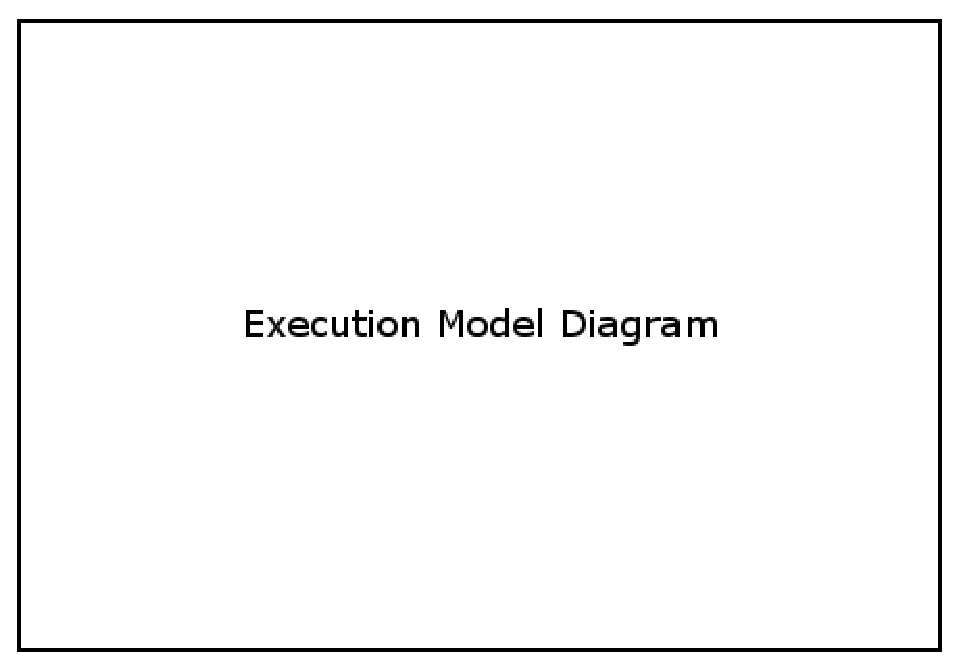
\includegraphics[height=6.2cm]{exmodel}
\caption{Model illustrating execution pattern of the new implementation}
\label{fig:exmodel}
\end{figure}

% A necessary overhead is incurred from the outset performing various initialisations discussed further in section 4.1. In 
% addition to this, the first chunk of data must be transferred to the device before the double buffering system can begin 
% to compensate for data transfer times. This initial transfer is carried out asynchronously while precomputing render 
% parameters such as those used in the 3d transformation, which will be static throughout the rendering process. The render 
% parameters are copied to the device, which subsequently begins rendering while the next chunk of data is transferred.

The first stage of rendering is a highly parallel 3D transform and colorize performed on a per-particle basis using 
four OpenMP threads per available core, to match the four available hardware threads, equating to roughly 240 threads. 
Transform parameters are precomputed, as they are the same for each particle, and computation is distributed amongst 
threads via an OpenMP parralel for loop. Further tuning enabled this loop to be auto-vectorized by the Intel compiler 
providing a large performance boost for this section.
% This stage is amenable to fast parallel processing and requires only a small amount of tuning for MIC suitability.

% The multistep OpenMP solution to the full rendering stage discussed in section [omp section] is modified to account for 
% the larger number of threads available. Simply splitting the image into smaller tiles to allow for more threads results 
% in particles affecting more tiles than previously, requiring more memory to store particle index lists per tile. To 
% account for this, the following approach is adopted. 

During a pre-render stage the number of available OpenMP threads are split into groups, the number of which is dependant on 
a runtime parameter, allocating a buffer per group for the resulting image. The dataset is evenly distributed amongst the 
groups, each rendering to the assigned buffers which are finally accumulated serially to a single image. 

Each group image is split into a two dimensional grid of tiles which are distributed amongst threads to avoid race 
conditions where multiple threads attempt to draw to a single pixel simultaneously. The number of tiles is determined 
through a user provided tile size parameter and the image size, and for each tile a list is generated containing the 
indices of all particles affecting the tile.

For the full render stage each thread processes a set number of tiles, rendering the list of particles for each tile. 
In this way pixels are not shared between threads and concurrent accesses are avoided. Finally when all 
chunks of data have been processed and accumulated, the resultant device image is copied back to the host for output. 


% Subsequent to group allocation, each thread group begins independently rendering an allocated subset of particles. This 
% occurs in two phases, a pre render phase and a render phase. In order to allow each thread sole access to a particular 
% set of pixels, and avoid race conditions discussed previously, the image is split into 2 dimensional grid of tiles – 
% the number of which is determined by a run time parameter tile\_size. The pre-render phase generates a list of particle 
% indices per tile, indicating all the particles whose area of influence overlaps with the tile. In this phase each thread 
% is allocated a subset of the group's allocated particles, and generates a list for each tile resulting in 
% (n\_thread * n\_tile) lists. A single thread accumulates the per-thread lists to attain a single list per tile. 
% Once all lists have been accumulated, phase two begins. In this phase each thread is allocated a tile, or subset of 
% pixels, and renders all particles in the list associated with that tile. In this way pixels are not shared between 
% threads and concurrent accesses are avoided.

% Following the accumulation of each group-specific image into a single buffer, which is retained throughout the entire 
% rendering process, the next chunk of data is processed until all particles have been rendered. This constant buffer is 
% then copied back to the host for output. 
%\medskip
%\noindent



\subsection{Optimisation}
\label{sect:micoptimisation}

% In order to appropriately exploit the MIC architecture and attain high performance gains, various optimisation methods 
% were explored. Some more generic methods are applicable to other similar architectures, such as Intel 64 and IA-32 [REF], while 
% others are specific to the Xeon Phi. 

\subsubsection{Memory Usage and Data Transfer}
\label{sect:memusage}

Cost of dynamic memory allocation on the Phi is relatively high [REF1], in order to minimise unnecessary allocations 
buffers are created at the beginning of the program cycle and reused throughout. Use of the MIC\_USE\_2MB\_BUFFERS 
environment variable forces buffers over a particular size to be allocated with 2MB pages rather than the default 4KB, 
which improves data allocation rate, transfer rate and can benefit performance by potentially reducing page 
faults and TLB (translation look-aside buffer) misses [REF2]. In tests using offload clauses for compiler 
managed memory allocation on the device, a single process offloading to the device and reserving large buffers allocated 
memory roughly 2-2.5x faster having set this environment variable to 64K. The inability to asynchonously allocate offload 
memory means overheads incurred allocating these buffers cannot be mitigated by overlapping allocation with host activity.

% initially allocated at approximately 4 to 4.5s per GB (with speed increasing marginally with increased allocation size). 
% Setting MIC\_USE\_2MB\_BUFFERS to 64K reduced this allocation overhead to approximately 2s per GB. [are approximations okay?]

Additionally, overheads in dynamic allocation and data transfer incur a penalty when running a single host process 
offloading to the device. In order to minimise these penalties, multiple MPI processes on the host are each allocated 
a subset of the device threads to exploit. In this way, the device is subdivided amongst the host MPI processes allowing 
for memory and data transfer to occur in parallel providing a noticeable performance increase, further details of which are 
given in sect. \ref{sect:results}.

% Often scientific datasets being visualized are very large, it is inevitable that there will at times be more data than 
% available device memory. This raises the issue of allocating and waiting for data transfer from main memory which, 
% while reaching roughly 6 GB/s over the 16 channel PCIe 2.0 connection, is an additional overhead to be considered.
% This is not such a large concern in a standard Intel 64 environment where frequent memory allocations, such as might be 
% invoked by repetitive resizing of dynamic arrays, have little comparative impact.

% Cost of dynamic memory allocation on the Phi is relatively high [REF1], in order to minimise unnecessary allocations 
% buffers are created at the beginning of the program cycle and reused throughout. Use of the MIC\_USE\_2MB\_BUFFERS 
% environment variable forces any buffers over a particular size to be allocated with 2MB rather than the default 4KB 
% pages, which improves data allocation rate, transfer rate and can benefit performance by potentially reducing page 
% faults and TLB (translation look-aside buffer) misses [REF2]. In isolated tests using offload clauses for compiler 
% managed memory allocation on the device, a single process offloading to the device and reserving large buffers 
% initially allocated at approximately 4 to 4.5s per GB (with speed increasing marginally with increased allocation size). 
% Setting MIC\_USE\_2MB\_BUFFERS to 64K reduced this allocation overhead to approximately 2s per GB. [are approximations okay?]

% Use of the offload syntax for asynchronous computation [REF?] allows to engage a double buffered approach, 
% processing the data in smaller chunks and overlapping computation and data transfer to minimise this overhead.

\subsubsection{Vectorization}
\label{sect:vectorization}

The large 512 bit width SIMD capability of the MIC architecture is exploited through vectorization carried out both 
automatically by the compiler, and manually using Intel Initial Many-Core Instructions (IMCI) [REF3]. Firstly the 
core data structure used in Splotch rendering was re-examined, and converted from an array of structures (AoS) to 
a structure of arrays (SoA). The AoS method stores a large array of structures, each containing all of the 
information pertaining to a single particle. This aids the compiler in automatic vectorization, 
amongst other changes such as ensuring the correct data alignment and modifying loops to be more easily vectorized 
as described in Intels Vectorization guide [REF 5] which, while providing examples for SSE, is applicable 
to IMCI as well. 

The rendering section of the algorithm is complex and unsuitable for automatic vectorization, this is manually 
optimised through use of the Intel intrinsics, which map directly to IMCIs. Drawing consists of additively 
combining a pixels current set of RGB values with the contribution from the current particle, which is calculated by 
multiplying the particle color by a scalar contribution value. In order to expedite this process, up to five single 
precision particle RGB values (totalling 480 bits) and five contribution values are packed into two respective 
512 bit vector containers. A third container contains 5 affected pixels, which are written simultaneously using a 
fused multiply add vector intrinsic, masked in order not to affect the final unused float value in the 16-float 
capable containers.

%  During rendering, each thread draws all particles affecting a particular subsection 
% of the final image. Particles are processed by drawing columns of affected pixels, from left to right, until all 
% affected pixels have been updated, illustrated in section [insert section or figure]. Drawing consists of additively 
% combining a pixels current set of RGB values with the RGB contribution from the current particle, which is calculated by 
% multiplying the particle color by a contribution value. In order to expedite this process up to five single 
% precision particle RGB values and five contribution values are packed into two respective 512 bit vector containers. 
% A third container contains 5 affected pixels, which are written simultaneously using a fused multiply add vector 
% intrinsic, masked in order not to affect the final unused float value in the 16-float capable containers. A 
% complex optimisation such as this is not likely to automatically occur during compiler optimisation, however 
% provides a performance increase for the rendering phase of up to 22\%.

% \subsubsection{MPI offload}
% \label{sect:mpioffload}

% The overheads in dynamic allocation and data transfer incur a significant penalty when running a single host process 
% offloading to the device. Data heavy algorithms such as Splotch require a lot of transfers, and ideally would use 
% as much of the device memory at a time as possible. One such solution to this problem is to run multiple host MPI 
% processes, each being awarded a subsection of the device to offload to and work with. This allows each process to 
% allocate a share of the memory, transfer subsections of data, compute and render the results asynchronously, thereby 
% utilising as much device memory as possible while minimising overheads. This provides a noticeable performance increase 
% discussed further in section [performance analysis sect], although must be implemented through a fairly unwieldy script 
% to distribute hardware threads amongst processes. [final sentence too opinionated?]

\subsubsection{Tuning}
\label{sect:tuning}

For smaller datasets where processing time is low, overheads regarding initialisation become no longer negligible. 
Initialisation of the device itself and OpenMP threads can cause a noticeable overhead. The impact of this can be 
minimised by placing an empty clause with empty OpenMP parallel section near to the beginning of the program, in order 
to overlap this overhead while other host activity is occurring, in this case while reading from file. Alternatively the 
environment variable OFFLOAD\_INIT can be set to on\_start to pre-initialise all available MIC devices before the program 
main begins execution. 

% Initialising the large number of OpenMP threads used on the device also carries a small overhead, roughly 0.3 seconds. 
% This can potentially be hidden though an empty parallel block, placed within an asynchronous offload section at the 
% beginning of the program. These two overheads are relatively small and may have little effect on a long running program, 
% however in a program expected to take only a few seconds to run they can outweigh any performance increase gained by 
% offloading to the device. It should be noted for a small program running many times over, as is the case when creating 
% a Splotch animation with a relatively small dataset, these overhead costs are paid only once during the first execution 
% as for repeat run-throughs Splotch execution is not actually stopped.

Various parameters of the algorithm can be tuned to find best performance. Rendering parameters such as the number of 
thread groups and tile size are set to optimal defaults for the test hardware based on results of scripted tests iterating 
through sets of incremental potential values. These can be modified via a parameter file passed in at runtime for differing 
hardware.

% The performance increase provided by running multiple MPI processes all offloading to subsections of the device is 
% notable. When offloading to the entire device with a single process, one of the debilitating factors was filling up 
% the device memory without wasting a large amount of time transferring this data. Building upon the pre-implemented MPI 
% Splotch functionality [ref to sect or ref], each process is allocated a subsection of the device via arguments to the 
% mpirun command, this  allows each process to independently allocate and transfer data to the device in parallel and 
% fill the device in a fraction of the time. The optimal number of processes for the test hardware was identified to be 
% eight, most likely due to the host socket for each device having eight-cores. [is this speculation bad?] 


\section{Performance Analysis}
\label{sect:performance}

Performance analysis consists of running a variety of tests on the available hardware, the “Dommic” facility at the 
Swiss National Supercomputing Centre, Lugano. Each node is based upon a dual socket eight-core Intel Xeon 2670 
processor architecture running at 2.6 GHz with 32 GB of main system memory. Two Xeon Phi 5110 MIC coprocessors are 
available per node. 

Tests are carried out using an N-Body simulation performed using Gadget [REF], consisting of roughly 21 million 
particles;  ~10 million dark matter particles, ~10 million baryonic matter particles and ~1 million star particles. 
A 100 frame animation orbiting the dataset is used to measure per-frame timings.

Both the host and device code use a tile size parameter of 100 pixels, while the device code has default parameters of 
8 host MPI processes, with 2 device threadgroups of 15 threads each, which has been shown in tests to be the optimal 
distribution for this hardware.

% The double buffered approach to data transfer and processing discussed in section [memory usage 3.3.1] allows to 
% process large sets such as this where the device memory is not sufficient to hold the entire dataset at one time. In 
% addition for smaller tests a filtering system in the file reader module allows just a subset of the data to be loaded.
% [update this with actual dataset size]

\subsection{Results}
\label{sect:results}

\begin{figure}
\centering
\includegraphics[height=6.2cm]{TotalTime}
\caption{Per-Frame rendering time using host with 1-16 cores vs host offloading to single and dual Xeon Phi devices}
\label{fig:totaltimes}
\end{figure}

Fig. \ref{fig:totaltimes} shows use of a single device provides comparable results to 4 cores on the host, while two devices outperform 
16 cores by 20\%. The additional use of a second device provides a 2x performance improvement for the MIC algorithm. 
Fig. \ref{fig:rotocol} shows the strongest area of improvement, the rototranslation and coloring phase, with a single device 
outperforming 16 cores roughly 2.5x, with roughly 3x improvement provided by using dual devices. The differing performances betweeen 
fig. \ref{fig:totaltimes} and fig. \ref{fig:rotocol} are due to the rendering phase, which does not gain as significant a 
performance boost as the roto-translation and coloring. 

\begin{figure}
\centering
\includegraphics[height=6.2cm]{Rotocol}
\caption{Per-Frame time to rototranslate and colorize test dataset using host with 1-16 cores vs single and dual Xeon Phi devices}
\label{fig:rotocol}
\end{figure}

Fig. \ref{fig:mpitimes} shows comparison of per-frame render times using varying numbers of MPI processes on the host, offloading to both a single and dual devices, 
shows best performance with 8 MPI processes per device, likely correspondant to the dual socket 8 core host CPU. 

\begin{figure}
\centering
\includegraphics[height=6.2cm]{MPIFrameTimes}
\caption{Per-Frame rendering time comparing 1-16 host MPI processes (per device) offloading to 1 and 2 Xeon Phi devices}
\label{fig:mpitimes}
\end{figure}



\section{Conclusions}
\label{sect:conclusions}

It can be seen from the results gathered so far that in some sections of code the MIC architecture excels well beyond the host, 
although in others a fair amount of modification is necessary to gain acceptable performance levels. The use of MPI on the host, 
despite implementation through an unwieldy execution script, provides a considerable performance increase especially for data heavy 
codes. 

Further work is planned to enable the code to run on multiple host nodess utilising all available devices, with further optimisation and 
testing to be done in order to perfect the double buffered data transfer and processing approach to effectively visualise much larger 
datasets. The ability to use multiple devices across multiple nodes will allow further testing of the scalability of the approach. 
Features provided in the new OpenMP 4.0 specification such as the \textit{teams} construct will enable a OpenMP based approach to 
threadgrouping as opposed to the manual method implemented here, if these constructs become supported by the Intel compiler in the future. 

Intel released details of their second generation Xeon Phi product, codenamed “Knights Landing”,  at the International Supercomputing 
Conference 2013 [ref]. One important factor to note is the potential to use this as a standalone CPU rather than a co-processor. 
This is worthy of further investigation as it invites the dismissal of complex and time consuming data transferral methods between 
a host and coprocessor, while retaining the ability to run directly on the host rather than copying executables to an external device.
%  One of the benefits of an offloading model is that work particularly suited to a highly 
% parallelised processing model can be offloaded while unsuitable work can be handled by the more powerful Xeon host 
% cores, disposal of the host would remove this advantage and beg the question of how to handle work that may be 
% inherently unsuitable for a many-core architecture.
 

\subsubsection{Acknowledgments.}

Acknowledge people and things here

%The following section shows a sample reference list with entries for
%journal articles \cite{jour}, an LNCS chapter \cite{lncschap}, a book
%\cite{book}, proceedings without editors \cite{proceeding1} and
%\cite{proceeding2}, as well as a URL \cite{url}.
%Please note that proceedings published in LNCS are not cited with their
%full titles, but with their acronyms!

\begin{thebibliography}{4}

\bibitem{jour} Smith, T.F., Waterman, M.S.: Identification of Common Molecular
Subsequences. J. Mol. Biol. 147, 195--197 (1981)

\bibitem{lncschap} May, P., Ehrlich, H.C., Steinke, T.: ZIB Structure Prediction Pipeline:
Composing a Complex Biological Workflow through Web Services. In: Nagel,
W.E., Walter, W.V., Lehner, W. (eds.) Euro-Par 2006. LNCS, vol. 4128,
pp. 1148--1158. Springer, Heidelberg (2006)

\bibitem{book} Foster, I., Kesselman, C.: The Grid: Blueprint for a New Computing
Infrastructure. Morgan Kaufmann, San Francisco (1999)

\bibitem{proceeding1} Czajkowski, K., Fitzgerald, S., Foster, I., Kesselman, C.: Grid
Information Services for Distributed Resource Sharing. In: 10th IEEE
International Symposium on High Performance Distributed Computing, pp.
181--184. IEEE Press, New York (2001)

\bibitem{proceeding2} Foster, I., Kesselman, C., Nick, J., Tuecke, S.: The Physiology of the
Grid: an Open Grid Services Architecture for Distributed Systems
Integration. Technical report, Global Grid Forum (2002)

\bibitem{url} National Center for Biotechnology Information, \url{http://www.ncbi.nlm.nih.gov}

\end{thebibliography}

%(REF7: Procedia Computer Science, 1(1) pp.1775-1784, 2010), and GPUs (REF8: Astronomical Society of the Pacific Conference 
%Series, 475 (ADASS XXII) pp.103-106, 2013; REF2: in preparation). 
%


\end{document}
